\documentclass[12pt,a4paper,oneside]{article}
\usepackage[utf8x]{inputenc}
\usepackage{ucs}
\usepackage[english]{babel}
\usepackage{dsfont}
\usepackage{mathtools}
\usepackage{amsfonts}
\usepackage{amssymb}
\usepackage{gensymb}
\usepackage{graphicx}
\usepackage{caption}
\usepackage{subcaption}
\usepackage{pgfplots}
\usepackage{hyperref}
\usepackage{booktabs}
\usepackage{float}
\usepackage{siunitx}
\usepackage{epstopdf}
\usepackage{amsmath} 
\usepackage{wrapfig}
\usepackage{fancyhdr}
\usepackage{lastpage}
\usepackage{pdfpages}
\usepackage{tocloft}
\usepackage{listings}

\definecolor{mGreen}{rgb}{0,0.6,0}
\definecolor{mGray}{rgb}{0.5,0.5,0.5}
\definecolor{mPurple}{rgb}{0.58,0,0.82}
\definecolor{backgroundColour}{rgb}{0.95,0.95,0.92}

\lstdefinestyle{CStyle}{
    backgroundcolor=\color{backgroundColour},   
    commentstyle=\color{mGreen},
    keywordstyle=\color{magenta},
    numberstyle=\tiny\color{mGray},
    stringstyle=\color{mPurple},
    basicstyle=\footnotesize,
    breakatwhitespace=false,         
    breaklines=true,                 
    captionpos=b,                    
    keepspaces=true,                 
    numbers=left,                    
    numbersep=5pt,                  
    showspaces=false,                
    showstringspaces=false,
    showtabs=false,                  
    tabsize=2,
    language=C
}

\tolerance=1500 % Denne gør at dine linjer ikke flyder ud i højre margin



\usepackage{xcolor}
\hypersetup{
    colorlinks,
    linkcolor={black},
    citecolor={blue!50!black},
    urlcolor={blue!80!black}
}

\pgfplotsset{compat=1.11}
\setlength\parindent{0pt}
\usepackage[a4paper]{geometry}
\geometry{
    left=3.5cm,  
    right=3.5cm,
    top=2.5cm, 
    bottom=2.5cm,
    headheight=\baselineskip,
    headsep=7mm,
    footskip=7mm
}
\linespread{1.4}
\counterwithin{equation}{section}
\counterwithin{figure}{section}

\setlength\cftparskip{-2pt}
\setlength\cftbeforesecskip{1pt}
\setlength\cftaftertoctitleskip{2pt}

\title{Exponential function PPNM}
\author{themjcricket }
\date{June 2021}
\title{The Exponential Function and an Approximation of this}
\author{Ajanthan Ketheeswaran Kumarasamy}

\begin{document}
\maketitle

\begin{abstract}
  This paper will briefly investigate the exponential function and an approximation of this. We will first look at the general form of an exponential function, then introduce the natural exponential function. We will then introduce an approximation of the exponential function and discuss why this function might work. Finally we will put the approximation to a test and see that it is a good approximation.
\end{abstract}
\section{Introduction}
The exponential	function is in general a function, where the argument of the function is the power of a	number ie. $f(x)=a \cdot b^{x}$, where $a$ is just a constant which satisfies, $f(0)=a$, since $b^{0}=1$. The derivative of the exponential function is given as
\begin{equation}
    \frac{d}{d x}b^{x} = b^{x} \ln{b}.
\end{equation}
Where $\ln{b}$ is the natural logarithm to $b$. However there is a unique base(or number so to say), $\text{e}=2.71828...$, which has the special property that,
\begin{equation}
    \frac{d}{d x}\text{e}^{x} = \text{e}^{x} \ln{\text{e}}= \text{e}^{x}.
\end{equation}
Which means that the derivative of the $\text{e}^{x}$ is just the function itself. This is known as the natural exponential function.
\section{Approximation Scheme}
The approximation scheme, which is used in this paper is,
\begin{lstlisting}[style=CStyle]
double ex(double x){
if(x<0)return 1/ex(-x);
return 1+x*(1+x/2*(1+x/3*(1+x/4*(1+x/5*(1+x/6*(1+x/7*(1+x/8*(1+x/9*(1+x/10)))))))));
}
\end{lstlisting}
If we first look at line 4 in the code, we can see that the approximation returns a value, which makes use of the fact that,
\begin{equation}
    \text{e}^{x}= \sum_{k=0}^{k=\infty}\frac{x^{k}}{k!}.
\end{equation}
However only to $k=10$. This would however only work for positive values, but the exponential function is also defined for negative values as, $\text{e}^{-x}=\frac{1}{\text{e}^{x}}$, which line 2 in the approximation takes care of. As you can see in Fig. \ref{fig:plot}, this approximation scheme only works for relatively low values of $x$. 
\begin{figure}[H]
  \centering
  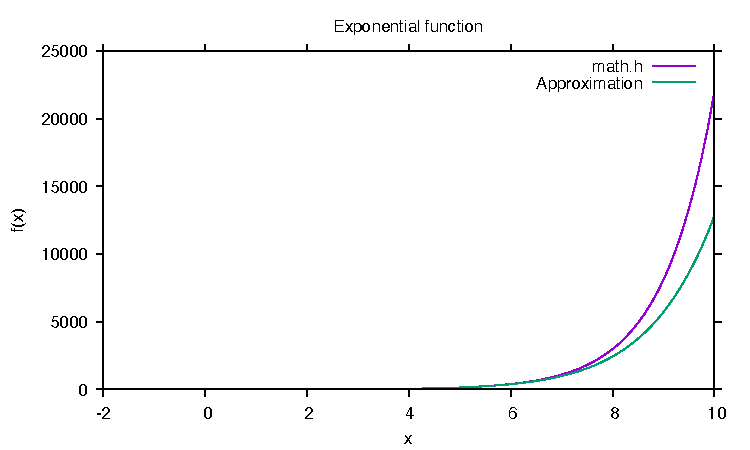
\includegraphics[width=\textwidth]{plot.pdf}
  \caption{Plot of the approximation scheme. It is plotted on top of the exponential function from math.h, where we see a noticeable deviation at around $x=7$.}
  \label{fig:plot}
\end{figure}
To ensure that larger values also follow the approximation, we include a new line to the approximation scheme as seen in here,
\newpage
\begin{lstlisting}[style=CStyle]
double ex(double x){
if(x<0)return 1/ex(-x);
if(x>1./8)return pow(ex(x/2),2);
return 1+x*(1+x/2*(1+x/3*(1+x/4*(1+x/5*(1+x/6*(1+x/7*(1+x/8*(1+x/9*(1+x/10)))))))));
}
\end{lstlisting}
Here we scale down values of $x>1/8$ to half of it and square the approximation (line 3 in the code), which as seen in Fig. \ref{fig:plot2} follows the exponential function well. I could not determine a value for which the approximation did not hold, which concludes that the approximation scheme is quite well.
\begin{figure}[H]
    \centering
    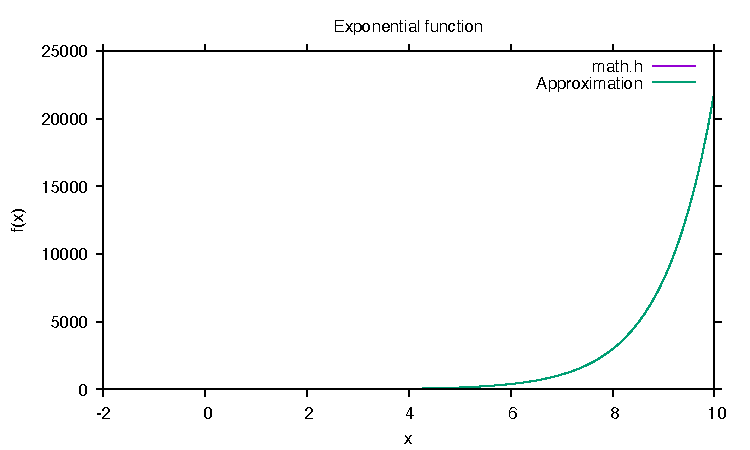
\includegraphics[width=\textwidth]{plot2.pdf}
    \caption{Plot of the final approximation scheme. It is plotted on top of the exponential function from math.h. We see that the two function follow each well. I have chosen not to include values greater than $x=10$, since I could not find a point, where the two functions deviated.}
    \label{fig:plot2}
\end{figure}

\end{document}
